\documentclass{assignment}

\usepackage{lipsum}

\newcommand*{\name}{}
\newcommand*{\id}{}
\newcommand*{\course}{Inferencia}
\newcommand*{\assignment}{Notas de clase 20 de Abril 2023}

\usepackage{amsmath,amssymb}

\newcommand{\Esp}{\mathbb{E}}
\newcommand{\Var}{\mathbb{V}ar}
\newcommand{\Prb}{\mathbb{P}}

\newcommand{\Nat}{\mathbb{N}}
\newcommand{\Rea}{\mathbb{R}}
\newcommand{\Rac}{\mathbb{Q}}
\newcommand{\Irr}{\mathbb{I}}

\begin{document}
\maketitle
\tableofcontents
\newpage

\section{Repaso matemático}
Sea $f:\mathbb{R} \to \mathbb{R}$ una función, decimos que la relación es lineal si $f$ se escribe como
\begin{align*}
    f(x)=ax+b
\end{align*}

\begin{figure}[h!]
    \centering
    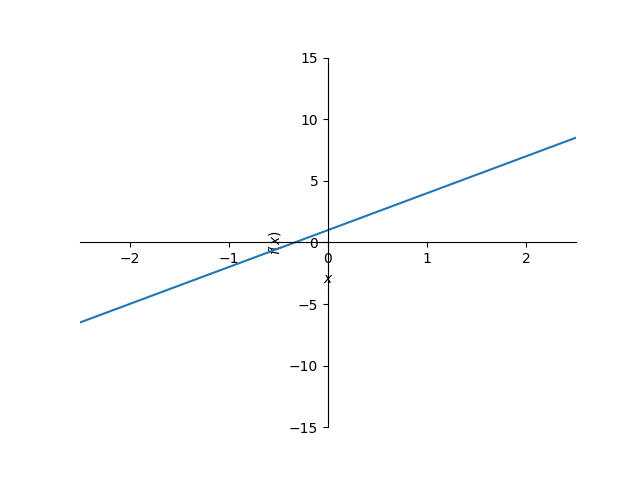
\includegraphics[scale=0.7]{lineal.png}
    \caption{función lineal}
    \label{fig:my_label}
\end{figure}
donde $a$ y $c$ son números reales y constantes. Las propiedades de las funciones lineales son muy útiles y bastante cómodas de usar. 

\textbf{Ejercicio:}
\begin{enumerate}
    \item Sean $f$ y $g$ funciones dadas por 
\begin{align*}
    f(x) & = 122x-123 \\ 
    g(y) &= 31y - \pi
\end{align*}
 \item Encuentra los números $x_0$ y $y_0$ de manera que $f(x_0)=0$ y $g(y_0)=0$. Calcula las funciones $f \circ g$ y $g \circ f.$
    \item Supongamos que tenemos un número $\alpha= a_1 x_1 + a_2 x_2 + a_3 x_3$ y una función 
    \begin{align}
        h(x) = \pi x - y\pi + e 
    \end{align}
    encuentra una expresión para $h(\alpha)$ en términos de  $h(x_1)$, $h(x_2)$ y $h(x_3).$

    \item  La esperanza es una función lineal. Consideremos las variables independientes $Z=X_1 Y_1 + X_2+Y_2$. Supongamos que estas variables aleatorias son idénticamente distribuidas e independientes. ¿Quién es $\Esp(Z)$? ¿Qué podemos decir si las funciones no son idénticamente distribuidas? 
    \item $\Esp(\Var(X))$ y $\Var(\Esp(X))$. 
    
\end{enumerate}

\section{Repaso}

Al proceso de estimar un parámetro mediante un número se llama \textbf{estimación puntual.} A la estimación de un parámetro mediante dos números entre los cuales se considera que debe estar el parámetro se llama estimación por intervalo del parámetro. 


Nos interesa saber si dada una muestra, que tenga media muestral entre $\mu - \varepsilon$ y $\mu + \varepsilon$ en un nivel de confianza del $95\%$, en términos de probabilidades es calcular,

\begin{align*}
   \Prb( \mu - \varepsilon < \overline{X} < \mu  +\varepsilon) = .95
\end{align*}

de manera equivalente

\begin{align*}
   \Prb( \overline{X} - \varepsilon < \mu < \overline{X} +\varepsilon) = .95
\end{align*}

cuando la muestra es muy grande, $\overline{X}$ tiene una distribución normal con media $\mu$ y varianza $\sigma^2/n$ y así 

\begin{align*}
   \Prb( \frac{- \varepsilon }{\sigma/\sqrt{n}} < \frac{\overline{X} - \mu }{\sigma/\sqrt{n}}  < \frac{\varepsilon }{\sigma/\sqrt{n}}) = .95
\end{align*}
por el teorema limite central tenemos que la distribución limite  $\overline{X}^*=\frac{\overline{X} - \mu }{\sigma/\sqrt{n}}$ es una $Norm(0,1)$.

\textbf{Ejemplo:}
Para medir el tiempo de reacción, un psicólogo estima que la desviación estándar es 0.05 segundos (s). ¿Qué
tan grande debe ser la muestra de las medidas para que se tenga una confianza: a) de $95\%$ y b) de $99\%$ en que el error de esta estimación no será mayor de 0.01 s?


\textbf{Ejercicio:}




\textbf{Ejercicio}


\textbf{Ejercicio:}



\textbf{Observaciones:}
\begin{enumerate}
    \item Notemos que $\varepsilon = \frac{1.96 \sigma}{\sqrt{n}}$. ¿Qué sucede cuando $n \to \infty$?
    \item De la tabla anterior. ¿Qué podemos decir cuando el error aumenta? Cierto o falso, la estimación por intervalos se hace menos precisa cuando mas confianza queremos. ¿Qué es mejor, una mejor estimación con menos confianza o mas confianza a costa de la aproximación?
    \item En caso de una muestra grande con media conocida pero varianza desconocida entonces se puede usar la desviación estándar $s^2$
\end{enumerate}

\section{$t$ de Student}
Cuando la muestra no es muy grande entonces $n/(n-1)$ no es despreciable y no podemos estar seguros que la desviación estándar aproxima a la varianza poblacional. Recordemos que una variable $t$ de Student se define como

\begin{align*}
t = \frac{\overline{X} - \mu}{S/\sqrt{n}}
\end{align*}
en este caso $S$ es la desviación estándar muestral, también para esta variable la distribución de $t$ no puede ser resulta por medios simple usamos tablas como el caso de la normal. Los grados de libertad es $n-1$ mientras que $n$ es el tamaño de la muestra. En este caso también tenemos intervalos de confianza. 


\textbf{Ejemplo:}
En cierto estado de la república, 9 estaciones meteorológicas ubicadas aleatoriamente encuentran que la precipitación pluvial en un mes determinado fue , en promedio, de $22$ cm con una desviación estándar de $3.5.$ Para la  precipitación media el   de confianza de $95\%$.

\end{document}